\chapter{Graphical Front End} % <<< ------------------------------------------ %
\label{ch:graphical_front_end}


To view measured data a graphical user interface (GUI in further text) was created. It can receive the recorded samples over the network and display them on a canvas. Furthermore it manages triggers and does a lot of math to get more specific metrics of a signal.
In this section the requirements for this piece of software, the design choices and the implementation details are discussed.

\section{Requirements}

The requirements for the GUI were given by the scope of Prof. Gut's 'Spektrum Analyzer' written in Java.
The task description required the new GUI to have the same features as the old one plus as many more as possible.

The requirements were as follows

\begin{itemize}
    \item Receive data over the network.
    \item Display received data in time as well as fequency space.
    \item Calculate the RMS power density in the signal.
    \item Calculate the THD ratio of the signal.
\end{itemize}

\section{Design Choices}

There is a wealth of programming languages to choose from. And there are as many libraries helping with graphics and networking as well for most of those languages.
In the following it is explained why we chose JavaScript and web technologies to implement a basic GUI.

In the comparison matrix \ref{fig:gui_language_choices} a select few popular possibilities were given weights for certain attributes of the respective language.

All the attributes are explained in the following.

\subsection*{Open Standard} Since this is a university based project meant for educational purposes too, it was very important to make all source code available under public license. Thus it was important to have a company and paid model independant sulution. Many languages are managed by a council or similar and open to public commits and thus deemed an open standard. Some are managed by a company and not classiefied as a open standard.

\subsection*{Networking} To ensure a fast and lossless data transfer, it was very important to have the choice between good networking protocols as well as convenient libraries to ease the use of those standards.
Networking is not a trivial thing and standards can be quite engineering and feature heavy. Thus it is important to have ready-to-use libraries that abstract the network. For more information on evaluated networking solutions, read Section \ref{TODO: networking}.

\subsection*{Graphics} An oscilloscope is quite requiring when it comes to graphics, since a image-stream that is fluent for the human eye has to be provided in a high resolution. This fact made it indispensable to use a library that interfaces OpenGL. Since a interface is not easy to design from scratch only using rectangles and circles, it was deemed important to have a GUI toolkit that makes the design process of the GUI easy. More on possible graphics libraries in section \ref{TODO: Graphics}

\subsection*{Widespread} It was important for the project to use a widespread solution since that way it is easy to obtain help and ask more savy users about certain pitfalls.

\subsection*{User-Friendly} Some solutions are more user-friendly when it comes to toolkit and usage. Since both team members come form a Linux background, it was strongly preferred to use a language that does not quasi-require a huge IDE or requires a lot of uneasy maintenance.

\subsection*{Easy To Use(r)} Since not all users want to fight with installers and package managers, the deployment options as well as general stability of the environment for the binaries were a strong point in the descision process.

\subsection*{Familiarity With The Language} The best toolkits do not matter if none of the involved programmers have ever used it and will struggle with even the basics for a major part of the project duration. Thus it was unavoidable to have some personal preferences for some languages.

\begin{table}
\begin{centering}
\setlength{\extrarowheight}{2pt}
\begin{tabular}{*{7}{c|}}
    \multicolumn{2}{c}{}        & \multicolumn{2}{c}{}\\\cline{3-7}
    \multicolumn{1}{c}{}    &   & \parbox[t]{2mm}{\rotatebox[origin=c]{90}{Rust}}%
                                & \parbox[t]{2mm}{\rotatebox[origin=c]{90}{C++}}%
                                & \parbox[t]{2mm}{\rotatebox[origin=c]{90}{Java}}%
                                & \parbox[t]{2mm}{\rotatebox[origin=c]{90}{Python}}%
                                & \parbox[t]{2mm}{\rotatebox[origin=c]{90}{JavaScript}} \\\cline{2-7}
                & Open Standard & 6 & 6 & 1 & 6 & 6\\\cline{2-7}
                   & Networking & 6 & 6 & 6 & 6 & 4\\\cline{2-7}
                     & Graphics & 2 & 5 & 5 & 5 & 6\\\cline{2-7}
                   & Widespread & 3 & 6 & 6 & 5 & 6\\\cline{2-7}
                & User-Friendly & 5 & 5 & 5 & 5 & 6\\\cline{2-7}
               & Easy To Use(r) & 3 & 4 & 5 & 6 & 6\\\cline{2-7}
& Familiarity With The Language & 3 & 4 & 3 & 6 & 6\\\cline{2-7}
                       & Total &28 &36 &31 &39 & 40\\\cline{2-7}
\end{tabular}
\caption{Weights of certain aspects of possible programming languages.}
\label{fig:gui_language_choices}
\end{centering}
\end{table}

After weighting in all the different aspects JavaScript was chosen as the language to implement the GUI for the oscilloscope. JavaScript is a scripting language that can be interpreted by the browser.
It is known for it's high versatility and widespread use in the web community.
A few years ago, JavaScript would not have been a viable choice for graphics and networking at all. But with the recent addition and more important great increase in stability in performance of WebGL and WebSockets, JavaScript has become a very potent solution available to everyone.
With JavaScript deploying the application to the enduser is as simple as making it accessible via a website that runs on the RedPitaya board. Thus it is very convenient for the user to work with the board, considering the assumption that every user has a webbrowser that is able to run the application.
A downside of JavaScript is the huge runtime the browser needs to execute the application and thus resulting in a lot of memory ressources used. Since those are easily available nowadays, this issue was considered non-relevant.
Another downside of JavaScript is that it leaves very little room when it comes to networking choices. For streaming data there is only WebSockets that performs well. Since WebSockets is a quite capable solution, this issue was also weighted rather light.

\subsection{Networking}

To ensure a fluent stream of data, very little overhead for the transmitted data is key.

Normally for streamed data where packets can be lost, \textbf{UDP} is the best choice since it has no overhead for guaranteeing completeness and in-order for all packets sent resulting in a packet header of only 2 bytes \cite{TODO: refrence}.
UDP sends packets but does not guarantee that none are lost. Since the scope only requires complete frames, those could be transmitted with a size of one UDP packet and thus ensuring no sample in the frame is lost. If no-lost-packets should be guaranteed, that would have been to implement.

For guaranteed transmission and sequentiality of the data, one is advised to use \textbf{TCP}. This comes at the cost of some more overhead resulting in a 6 byte header \cite{TODO: refrence}. Considering the huge packet size this header is, with less than 0.1 \% of the total packet size, completely negligible. What TCP does more and was important for this project is congestion control. It ensures that no more packets are sent if old ones are missing. It prevents the network from collapsing because an UDP sender sends all packets it can and thus using the entire bandwidth even if the receiver cannot even process the data at this point.
This means that TCP also helps when the bandwith is small by waiting for the current package and not already sending further packages and thus providing sort of automatic bandwith adaption.
There is the possibility of using raw TCP sockets or one of TCP's subprotocols. Raw sockets require the user to implement their own protocol entirely to handle data transmission on an application layer whilst using subprotocols already provide a standard way to do so.
Two of those subprotocols are HTTP and WebSockets. HTTP comes with great overhead and is meant for single transactions only.
WebSockets on the contrary are meant for data streaming.
Since JavaScript enforces WebSockets the functionality is explained a little bit more in the following.

\subsubsection{WebSockets}

WebSockets final RFC 6455\cite{TODO: https://tools.ietf.org/html/rfc6455,} was released in December 2011 and is thus still quite young. It is meant to compensate the lack of raw UDP and TCP sockets in JavaScript which is due to security threats that are not further elaborated here.
WebSockets is located in the Application Layer of the OSI model\footnote{TODO: https://en.wikipedia.org/wiki/OSI\_model}.
Instead of opening a raw WebSocket, the handshake is done via HTTP(S). This brings the benefit of communicating through the same ports as the browser (80 or 443) which enables the protocol to go through most firewalls.
The client sends an upgrade request to the server which then opens a WebSocket connection.
This allows for a very conventient way to use TCP Sockets without any entirely new standards.
The section "1.5 Design Philosophy" in the RFC 6455\cite{TODO: https://tools.ietf.org/html/rfc6455,} explains it very well:
Basically it is intended to be as close to just exposing raw TCP to script as possible given the constraints of the Web.

The only exception is that WebSockets adds framing to make it packet rather than stream based and to differentiate between binary and text data.
This differentiation is very useful for this project. Instructions to the server are issued via the text channel whilst data is sent back through the binary channel, allowing for very convenient interfacing with close to no effort.

\subsection{Graphics}

The graphics portion of the GUI is the most important part. Since the GUI should plot data fast and conveniently as well as display some numbers and provide controls to manipulate the view, it is important to have a good library, that enables all those things. It is absolutely key to render the graphics on the GPU. Since the application should be cross platform and open source, libraries using OpenGL are a good choice.

With the choice of JavaScript \& HTML there comes a great wealth of libraries that enable the user to easily write GUI applications. Prototyping is fast and with CSS and a lot of different frameworks the GUI is also nice-looking.

A few frameworks were evaluated to build the controls of the scope, with mithril.js finally being chosen for it's simplicity and flexibility. Mithril is a framework with an exceptionally low footprint and high DOM recalculation.
Those two facts are key to a good WebUI, since the User does not want to load lots of data and also does not want to experience any lag when building up the UI again.
More on mithril.js in section \ref{TODO: mithril.js}.

To plot the data some graphing libs could have been used. Those would namely be plotly.js or chart.js. Whilst they bring in a lot of built in functionality like logarithmic plots or automatic axis labeling, they also have a quite heavy overhead.
Practical experience and tests have shown that both of them are not meant and performant enough to plot high amounts of data in real time.
Thus it was decided to use WebGL draw calls directly to draw on a HTML canvas. A HTML canvas is an environment that is directly exposed from the GPU to the user such that he can use GPU rendering inside the browser.
More on WebGL and it's functioning in section \ref{WebGL}

\section{Implementation}

\subsection{WebGL}

% \begin{figure}
%     \centering
%     %\section{Scope}

\begin{frame}
    \frametitle{Demo}

    \centering
    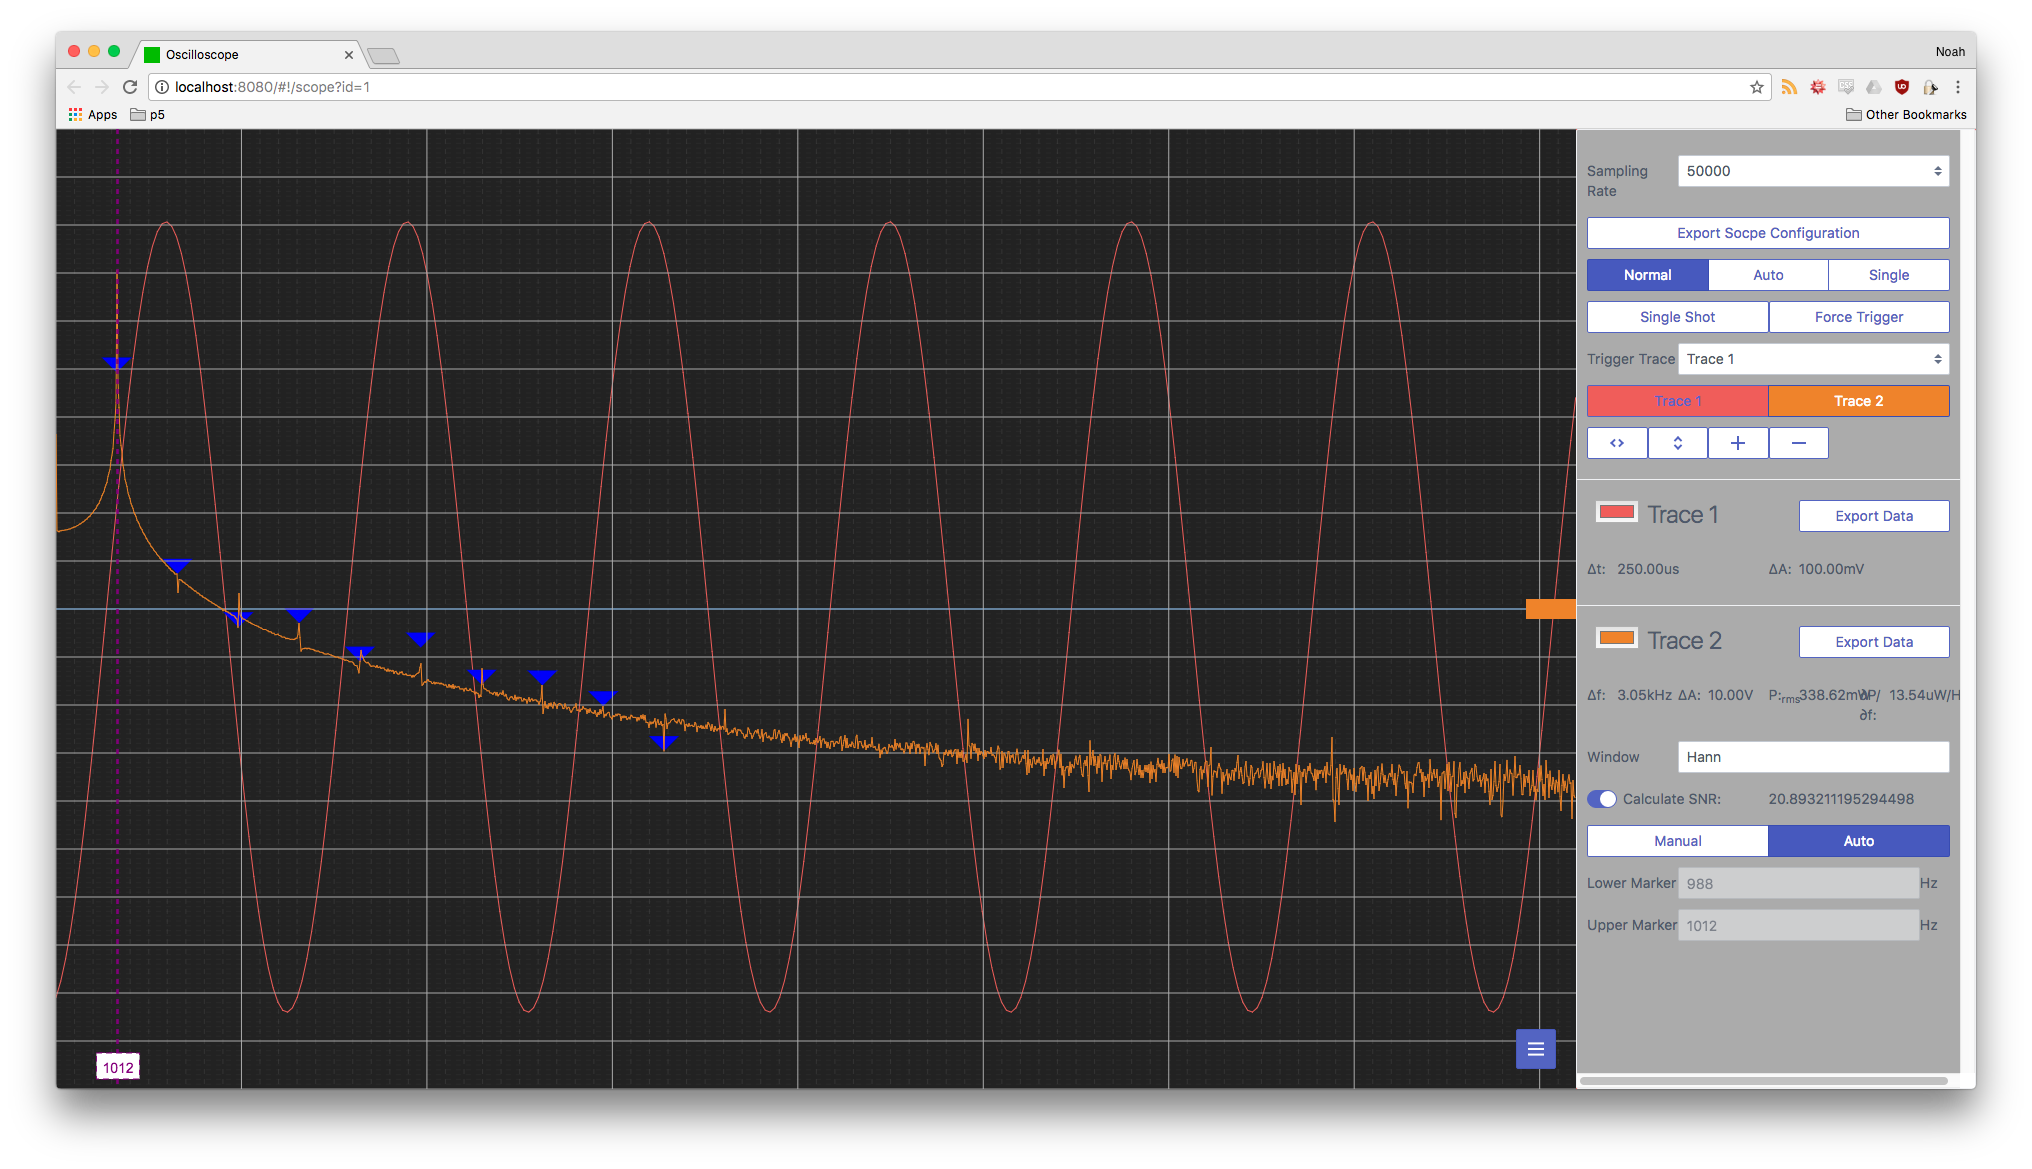
\includegraphics[width=1\textwidth]{images/scope}
\end{frame}

\begin{frame}
    \frametitle{Technologies used}

    \centering
    \begin{tikzpicture}
        \node at (0,0) {
\includegraphics[width=2cm]{images/logos/JS.jpeg}};
        \node at (4,-1) {
\includegraphics[width=2cm]{images/logos/webgl.jpeg}};
        \node at (0,-4) {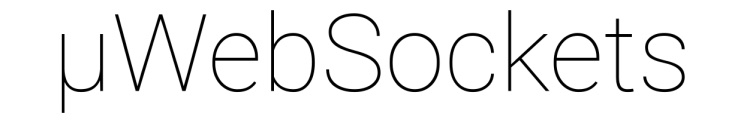
\includegraphics[width=2cm]{images/logos/uws.jpeg}};
        \node at (4,-4) {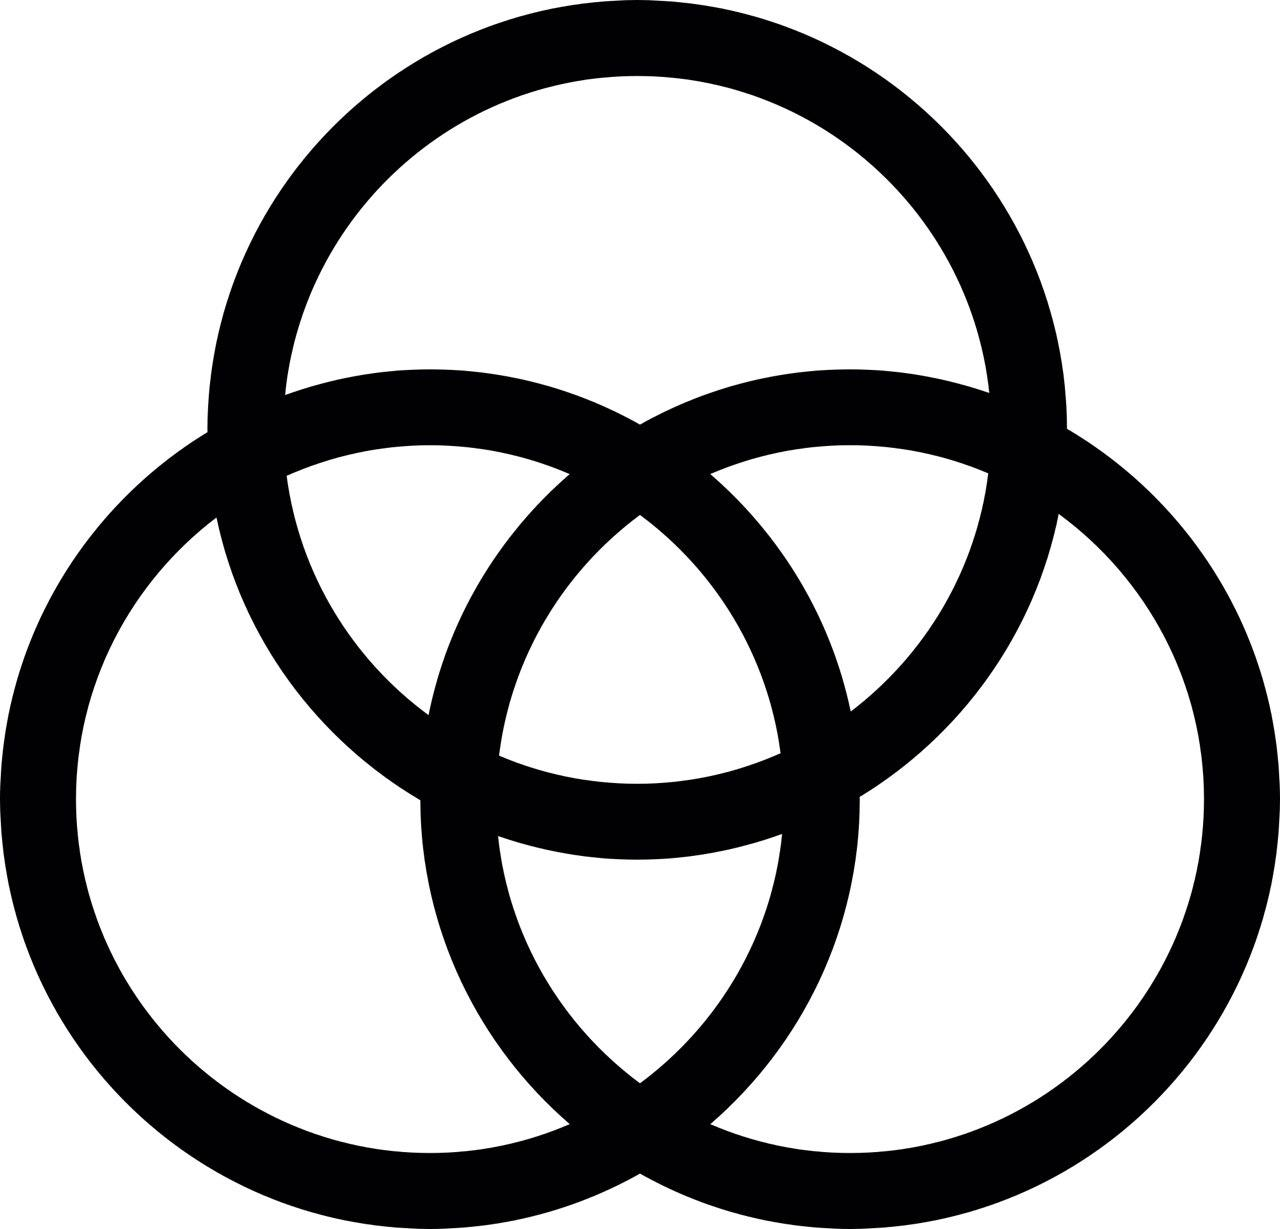
\includegraphics[width=2cm]{images/logos/mithril.png}};
    \end{tikzpicture}
\end{frame}

%     \caption{Digital signal processing chain from analog signal to the digitally processed data stream}
%     \label{fig:filtertopologies:cic}
% \end{figure}

The application uses the canvas dom element which provides a direct interface to WebGL. The user can render vertices to the canvas and apply shaders.
In the case of this application simple 2D calls suffice since it is essentially only necessary to draw lines.
Via the canvas one can retreive a 2D Rendering Context on which simple geometry can be drawn directly.
In JavaScript this can be done using the code in \ref{lst:js2dcontext} which shows how a single red line can be drawn on the canvas.

\begin{tcolorbox}[
        title={
            \refstepcounter{listing}
            Listing \thelisting: JavaScript ``Get 2D Rendering Context''
            \label{lst:js2dcontext}
            \addcontentsline{lol}{listing}{\protect\numberline{\thelisting}}
        }
    ]
    \begin{minted}[
        linenos,
        numbersep=4pt,
        style=solarizedlight,
    ]{javascript}
        // Get the canvas element from the dom
        var canvas = document.getElementById('canvas-id');
        // Get the 2d context of the canvas
        var context = canvas.getContext('2d');

        // Set brush color to red
        context.strokeStyle = '#FF0000';

        // Start a new path and move the cursor
        // from start to end of the line to be drawn
        context.beginPath();
        context.moveTo(x, y);
        context.lineTo(x + 100, y + 100);

        // Finally actually draw the line on the canvas and end the path
        context.stroke();
    \end{minted}
\end{tcolorbox}

There is also the possibility to draw rectangles, circles and much more. All of those elements can be styled easily via properties of the context environment.

Now we are able to draw something on a canvas once. If this should be done to create an actually moving image, those draws on the canvas have to be done over and over again. There is various possibilities to do that in JavaScript but only one is actualy performant and recommended. Instead of just drawing to the canvas over and over again, it would be ideal to only do that before a new frame is pulled from the framebuffer by the display. JavaScript provides a interface to register a callback that is called before a new frame is released. This callback will be called with the same frequency as the display referesh rate, which nowadays usually is \SI{60}{\hertz}.
To make sure that callback will always be executed it has to be registered again after a callback was issued. The sample \ref{lst:jsglcallback} shows this is done conveniently.

\begin{tcolorbox}[
        title={
            \refstepcounter{listing}
            Listing \thelisting: JavaScript ``Get 2D Rendering Context''
            \label{lst:js2dcontext}
            \addcontentsline{lol}{listing}{\protect\numberline{\thelisting}}
        }
    ]
    \begin{minted}[
        linenos,
        numbersep=4pt,
        style=solarizedlight,
    ]{javascript}

        // The register function is not named the same way in every browser
        // Make sure this is the case
        window.requestAnimationFrame = window.requestAnimationFrame
                                    || window.webkitRequestAnimationFrame;

        // Our callback we call for every frame drawn
        export const draw = function() {
            // Draw anything needed

            // End draw

            // Register the callback again
            requestAnimationFrame(function(){
                // Execute our callback
                // We cannot hand this directly to the register function
                // since it is not yet known inside it's own definition
                draw();
            });
        };

        // Initially call the draw function
        draw();
    \end{minted}
\end{tcolorbox}

This callback will not affect the rest of the DOM. Like that the JavaScript Runtime will handle the redraws of the dom performantly whilst the callback will render a fluent graph of the data.

\subsection{mithril.js}

TODO: how do we work with mithril.js (basic concepts, important to know, code-samples)

The official mithril webpage describes mithril.js the following way: ``Mithril is a modern client-side Javascript framework for building Single Page Applications. It's small (< 8kb gzip), fast and provides routing and XHR utilities out of the box.'' \cite{TODO: mithril.js.org}. Mithril, like a lot of other frameworks like React, Angular.js or Vue.js uses a virtual DOM. This means that it does not modify the DOM the browser outlines but rather maintains it's own DOM. When a new render call is issued, the virtual DOM calculates all the deltas that stem from new content and applies them. Like this mithril.js performantly calculates the DOM based on a descriptive model. The developer does not have to manually modify an objects state but rather describes it.

A redraw generally happens when an event is triggered by any input element but can also be issued manually.
A virtual DOM consists of many vnodes and can be mounted on any node of the browser's DOM as example \ref{lst:jsmithrilmount} shows.

\begin{tcolorbox}[
        title={
            \refstepcounter{listing}
            Listing \thelisting: JavaScript ``Get 2D Rendering Context''
            \label{lst:js2dcontext}
            \addcontentsline{lol}{listing}{\protect\numberline{\thelisting}}
        }
    ]
    \begin{minted}[
        linenos,
        numbersep=4pt,
        style=solarizedlight,
    ]{javascript}

        // A mithril component is a simple object that has at minimum a
        // view() function that returns a vnode.
        var HelloWorld = {
            view: function() {
                // Return the toplevel <div> vnode
                return m('', [
                    // Create a <h1> vnode with the attribute class="title"
                    m('h1', { class: 'title' }, 'A very interesting title!'),
                    // Create a <p> vnode
                    m('p', 'Hello World!'),
                ])
            }
        }
        // Get the root div and mount the HelloWorld component
        var root = document.getElementById('root');
        m.mount(root, HelloWorld)
    \end{minted}
\end{tcolorbox}

A component can be mounted on any DOM node and becomes a vnode in the virtual DOM. The developer can create new Components by simply creating an object that holds at least a view() function that instantiates new vnodes.
The new Component can then be instantiated via the m() or m.mount() command.
As this section should only give a base overview on mithril and is not meant to be a manual, further information on mithrils features and usage can be obtained on it's webpage\footnote{TODO:https://mithril.js.org}.

TODO: https://mithril.js.org/vnodes.html
TODO: https://mithril.js.org/

\subsection{WebSockets}

To receive data over the network, WebSockets are used. WebSockes could be explained as bare TCP sockets whose connection is initiated via HTTP.
JavaScript provides a very easy to use interface which makes it really easy to shove data back and forth.
As anything in JavaScript this again is done using callbacks. There is callbacks that handle connections, messages and errors. All the details can be read in the Mozilla documentation \cite{TODO: https://www.html5rocks.com/en/tutorials/websockets/basics/}. The code snippet in \ref{lst:TODO:} should give only a short hint how WebSockets in JavaScript are used.

\begin{tcolorbox}[
        title={
            \refstepcounter{listing}
            Listing \thelisting: JavaScript ``Get 2D Rendering Context''
            \label{lst:js2dcontext}
            \addcontentsline{lol}{listing}{\protect\numberline{\thelisting}}
        }
    ]
    \begin{minted}[
        linenos,
        numbersep=4pt,
        style=solarizedlight,
    ]{javascript}

        // Open a new socket
        this.socket = new WebSocket('ws://localhost');
        // Make sure the binary data transmitted
        // is interpreted as an ArrayBuffer
        // More on ArrayBuffers and Blobs in:
        // - https://developer.mozilla.org/en/docs/Web/API/Blob
        // - https://developer.mozilla.org/en-US/docs/Web/JavaScript/Reference/Global_Objects/ArrayBuffer
        this.socket.binaryType = 'arraybuffer';

        // Define all the callback handlers
        connection.onopen = function () {
            // The connection was established; send some regards.
            connection.send('Hello World!');
        };

        connection.onerror = function (error) {
            // An error has occurred; print it to the console.
            console.log('WebSocket Error: ' + error);
        };

        connection.onmessage = function (e) {
            if (typeof e.data == 'string') {
                // If a text type message was received, print it out.
                console.log('Text message received: ' + e.data);
            } else {
                // A binary type message was received.
                // Interpret the values as 16 bit uints.
                var arr = new Uint16Array(e.data);
                // Plot the data.
                plot(arr);
            }
        };
    \end{minted}
\end{tcolorbox}

TODO: how do we work with websockets (important callbacks, code-samples)

\subsection{Application Structure}

The entire application consists of a single state tree that should make it very easy to import and export settings as well as concentrate all the states in one place which gives a way better overview than in the case all the states are scattered in various objects in the application.
Listing \ref{lst:app_structure} shows an extract of the tree structure.

\begin{tcolorbox}[
        title={
            \refstepcounter{listing}
            Listing \thelisting: JavaScript ``Get 2D Rendering Context''
            \label{lst:js2dcontext}
            \addcontentsline{lol}{listing}{\protect\numberline{\thelisting}}
        }
    ]
    \begin{minted}[
        linenos,
        numbersep=4pt,
        style=solarizedlight,
    ]{javascript}

        var appState = {
            scopes: [{
                id: 1,
                name: 'Scope ' + 1,
                top: 250,
                left: 350,
                mode: 'normal',
                ui: {
                    mover: {
                        width: 50,
                        height: 20,
                        horizontalPosition: 0,
                    },
                    prefPane: {
                        open: true,
                        width: 400,
                    }
                },
                source: {
                    id: 2,
                    name: 'Source ' + 1,
                    top: 300,
                    left: 50,
                    location: 'ws://localhost:50090',
                    frameSize: 4096,
                    samplingRate: 5000000,
                    bits: 16,
                    vpp: 2.1, // Volts per bit
                    buffer: {
                        upperSize: 4,
                        lowerSize: 1,
                    },
                    trigger: {
                        type: 'risingEdge',
                        level: 0,
                        channel: 1,
                        hysteresis: 30,
                        slope: 0
                    },
                    triggerTrace: 0,
                    triggerPosition: 1 / 8,
                    numberOfChannels: 2,
                    mode: 'normal',
                    activeTrace: 0,
                    traces: [
                        {
                            id: 4,
                            offset: { x: 0, y: 0 },
                            windowFunction: 'hann',
                            halfSpectrum: true,
                            SNRmode: 'auto',
                            info: {},
                            name: 'Trace ' + 2,
                            channelID: 1,
                            type: 'FFTrace',
                            color: '#E8830C',
                            scaling: {
                                x: 1,
                                y: 1,
                            },
                            markers: [
                                {
                                    id: 'SNRfirst',
                                    type: 'vertical',
                                    x: 0,
                                    dashed: true,
                                    color: 'purple',
                                    active: true,
                                },
                                {
                                    id: 'SNRsecond',
                                    type: 'vertical',
                                    x: 0,
                                    dashed: true,
                                    color: 'purple',
                                    active: true,
                                },
                            ]
                        }
                    ],
                }
            }]
        };
    \end{minted}
\end{tcolorbox}

All of the values that can be controlled through the GUI - and many more - are also controllable directly through the state tree.
On application start the entire statetree is loaded. TODO: export function


TODO: basic structure of the application

\subsection{Power Calculation}

TODO: how do we calculate rms power and the power density spectrum

\subsection{SNR Autodetection}

TODO: how do we calculate the snr (incl. windowing etc)

\subsection{THD Calculation}

TODO: how do we calculate THD

\section{Product}

TODO: images, features, etc

% >>>

%^^A vim: foldenable foldcolumn=4 foldmethod=marker foldmarker=<<<,>>>
